\documentclass{article}


% if you need to pass options to natbib, use, e.g.:
%     \PassOptionsToPackage{numbers, compress}{natbib}
% before loading neurips_2024


% ready for submission
%\usepackage{neurips_2024}


% to compile a preprint version, e.g., for submission to arXiv, add add the
% [preprint] option:
% \usepackage[preprint]{neurips_2024}


% to compile a camera-ready version, add the [final] option, e.g.:
\usepackage[final]{neurips_2024}


% to avoid loading the natbib package, add option nonatbib:
%    \usepackage[nonatbib]{neurips_2024}


\usepackage[utf8]{inputenc} % allow utf-8 input
\usepackage[T1]{fontenc}    % use 8-bit T1 fonts
\usepackage{hyperref}       % hyperlinks
\usepackage{url}            % simple URL typesetting
\usepackage{booktabs}       % professional-quality tables
\usepackage{amsfonts}       % blackboard math symbols
\usepackage{nicefrac}       % compact symbols for 1/2, etc.
\usepackage{microtype}      % microtypography
\usepackage{xcolor}         % colors
\usepackage{tabularx}
\usepackage{booktabs}


\title{How You Distinguish People by Voice}


% The \author macro works with any number of authors. There are two commands
% used to separate the names and addresses of multiple authors: \And and \AND.
%
% Using \And between authors leaves it to LaTeX to determine where to break the
% lines. Using \AND forces a line break at that point. So, if LaTeX puts 3 of 4
% authors names on the first line, and the last on the second line, try using
% \AND instead of \And before the third author name.


\author{%
	Pu Fanyi\thanks{Equal Contribution} \hspace{1em} Jin Qingyang\footnotemark[1] \hspace{1em} Soo Ying Xi\footnotemark[1] \hspace{1em} Shan Yi\footnotemark[1] \hspace{1em} Zhang Xintong\footnotemark[1] \\
	School of Computer Science and Engineering\\
	Nanyang Technological University\\
	Singapore 639798 \\
	\texttt{\{FPU001, JINQ0003, D220001, SH0005YI, XZHANG113\}@e.ntu.edu.sg} \\
}

\usepackage{graphicx}

\begin{document}
	
	\begin{titlepage}
	\begin{figure}[!t]
		\centering
		
\includegraphics[width = 4.3in]{title/logo.pdf}
	\end{figure}
	
	\centering
	\huge{\textbf{MH3511: Data Analysis with Computer}}\\[0.2in]
	\huge{\textbf{Project Report}}\\[2in]
	
	%	\LARGE{\textbf{YOUR NAME}}\\
	%	\normalsize{Matriculation number}\\[0.2in]
	
	\begin{table}[h]
		\centering
		\resizebox{\textwidth}{!}{%
			\begin{tabular}{lll}
				\toprule
				\textbf{Name} & \textbf{Email} & \textbf{Matric Number} \\
				\midrule
				Pu Fanyi & FPU001@e.ntu.edu.sg & U2220175K \\
				Jin Qingyang & JINQ0003@e.ntu.edu.sg & U2220239A \\
				Soo Ying Xi & D220001@e.ntu.edu.sg & U2220021D \\
				Shan Yi & SH0005YI@e.ntu.edu.sg & U2222846C\\
				Zhang Xintong & XZHANG113@e.ntu.edu.sg & U2210809G\\
				\bottomrule
			\end{tabular}%
		}
	\end{table}
	
	\Large{Course Coordinator: Dr. Yue Mu}\\[0.5in]
	
	%	\large{A Final Year Report submitted to Asian School of the Environment, Nanyang Technological University in partial fulfilment of the requirements for the Degree of }\\[0.1in]
	
	\LARGE{School of Computer Science and Engineering}\\
	\LARGE{Nanyang Technological University, Singapore}\\[0.3in]
	
	
	\LARGE{2023/2024 Semester 2}
	\newpage
\end{titlepage}
	\newpage
	
	
	\maketitle
	
	
	\begin{abstract}
		Advancements in artificial intelligence (AI) have revolutionized various domains, including speech synthesis. The ability to generate human-like voices using AI has immense potential applications, from virtual assistants to entertainment media. It's essential to understand the nuances and characteristics of human speech, including variations influenced by gender. By examining datasets encompassing a wide range of voices, we aim to uncover insights into the distinct patterns and distributions of voice frequencies across genders. Though the available voice samples remain unprocessed and unrefined, our objective is to explore the correlation between voice frequency data attributes—such as mean frequency, standard deviation, median frequency, Q25 frequency, Q75 frequency, skewness, mean fundamental frequency—and the gender or age group of the respective voice sample.
	\end{abstract}
	
	
	\section{Introduction}
	Gender and age play a significant role in shaping the fundamental characteristics of vocal communication. Recognizing and understanding these differences is crucial for developing AI systems capable of producing voices that resonate authentically with diverse audiences. With more and more open-source voice samples available online today, we extract the data from voice samples, with further analysis to gain more insight into this topic. Although the available voice samples remain unprocessed and unrefined, our objective is to explore the correlation between voice frequency data attributes and gender or age group of the respective voice sample.
	
	In our project, a dataset comprising labels indicating gender and age group alongside various voice frequency attributes is used. Our group downloaded open-source voice samples from the internet and further extracted diverse voice frequency attributes to compile this dataset.
	
	Based on this dataset, we seek to answer the following questions:
	\begin{enumerate}
		\item Is there a notable discrepancy in mean frequency between male and female voices?
		\item Does the gender of a voice sample correlate with its mean fundamental frequency?
		\item Are there distinct variations in standard deviation between voices of different genders?
		\item Can gender be discerned by examining the quantiles of voice frequency data?
	\end{enumerate}
	
	This report will cover the data descriptions and analysis using R language. For each of our research objectives, we performed statistical analysis and drew conclusions in the most appropriate approach, together with explanations and elaborations.
	
	
	\section{Data Preparation}
	
	\subsection{The DiffVoice Dataset}
	
	In order to analyse the relationship between voice features and the information of the speaker, DiffVoice is created for analysis. We collected the raw voice data with captions from Common Voice (cite) English subset, with different genders, regions and ages.
	
	The feature extraction pipeline for voice data involves the following steps:
	\begin{enumerate}
		\item \textbf{Audio Loading}: Raw audio files are loaded and converted into waveforms.
		\item \textbf{Preprocessing}: Audio is normalized and resampled to a consistent format.
		\item \textbf{Feature Extraction}: Key features such as Mel-frequency cepstral coefficients (MFCCs), spectral centroid, spectral entropy, spectral flatness, pitch, and magnitude are extracted.
		\item \textbf{Statistical Aggregation}: Statistical measures like mean, standard deviation, and median are calculated for features extracted.
	\end{enumerate}
	
	This pipeline transforms raw voice recordings into a set of numerical descriptors that capture the essential qualities of the audio for analytical tasks.
	
	The descriptions of the extracted features have been listed in Table ~\ref{table:features_description}.
	
	{
		\renewcommand{\arraystretch}{1.3}
		\begin{table}
			\centering
			\begin{tabular}{lll}
				\hline
				\textbf{Feature Name} & \textbf{Feature Description} & \textbf{Feature Type} \\
				\hline
				\texttt{meanfreq} & Average frequency (kHz) & Continuous Variable \\
				\texttt{sd} & Frequency standard deviation & Continuous Variable \\
				\texttt{median} & Median frequency (kHz) & Continuous Variable \\
				\texttt{Q25} & First quartile (kHz) & Continuous Variable \\
				\texttt{Q75} & Third quartile (kHz) & Continuous Variable \\
				\texttt{IQR} & Interquartile range (kHz) & Continuous Variable \\
				\texttt{skew} & Skewness of the frequency distribution & Continuous Variable \\
				\texttt{kurt} & Kurtosis of the frequency distribution & Continuous Variable \\
				\texttt{sp.ent} & Spectral entropy & Continuous Variable \\
				\texttt{sfm} & Spectral flatness measure & Continuous Variable \\
				\texttt{mode} & Mode frequency & Continuous Variable \\
				\texttt{centroid} & Frequency centroid & Continuous Variable \\
				\texttt{meanfun} & Mean fundamental frequency across the signal & Continuous Variable \\
				\texttt{minfun} & Minimum fundamental frequency across the signal & Continuous Variable \\
				\texttt{maxfun} & Maximum fundamental frequency across the signal & Continuous Variable \\
				\texttt{meandom} & Mean dominant frequency across the signal & Continuous Variable \\
				\texttt{mindom} & Minimum dominant frequency across the signal & Continuous Variable \\
				\texttt{maxdom} & Maximum dominant frequency across the signal & Continuous Variable \\
				\texttt{dfrange} & Dominant frequency range & Continuous Variable \\
				\texttt{modindx} & Modulation index & Continuous Variable \\
				\texttt{age} & Age of the speaker & Ordinal Variable \\
				\texttt{gender} & Gender of the speaker & Nominal Variable \\
				\texttt{accent} & Accent of the speaker & Nominal Variable \\
				\hline
			\end{tabular}
			\caption{Description of Features}
			\label{table:features_description}
		\end{table}
	}
	
	We organized the dataset into CSV files and uploaded it onto HuggingFace for easier visualization and management.
	
	Before proceeding with data analysis, preliminary data cleaning was performed to achieve the following:
	\begin{enumerate}
		\item Irrelevant columns such as ``accents'' are eliminated from the data set
		\item The ``country'' attribute is dropped as it is out of the scope of our project.
	\end{enumerate}
	
	
	\subsection{Data Preparation}
	\begin{figure}
		\centering
		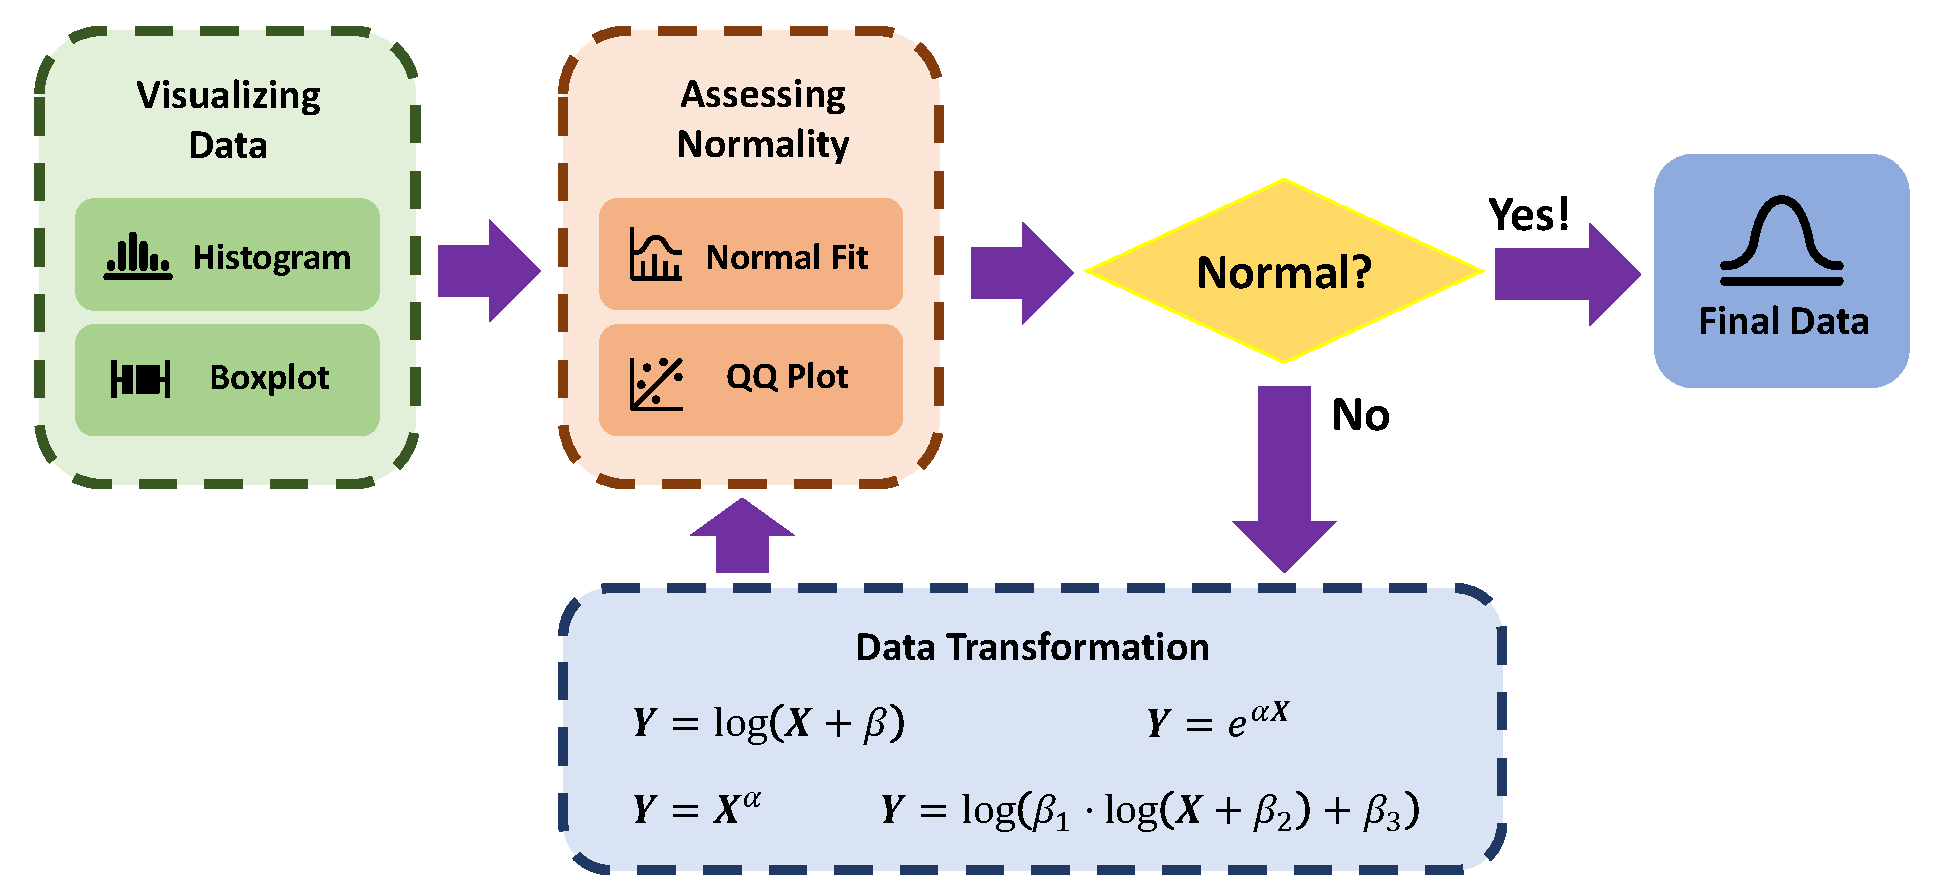
\includegraphics[width=\textwidth]{graphs/prepare_data.pdf}
		\caption{The pipeline for data preparation.}
		\label{data_prep}
	\end{figure}
	The data preparation process starts with:
	\begin{enumerate}
		\item Gaining a basic understanding of the data distribution using histogram. This visual representation easily allows us to assess the skewness or symmetry of these distributions.
		\item The mean and standard deviation are then calculated for each attribute, giving us an idea of the central tendency and dispersion of the data. 
		\item We then proceed to assess the normality of data using QQ-plot, deviation from the reference line indicates that the data is not normal. In that case, we will apply logarithmic transformation to normalize some features of the data. 
		\item Followed by log transformation, we defined a function \texttt{get\_outlier} to extract the outliers. We examined the total number of outliers identified across different columns and found that the percentage of outliers is less than 5\%. Thus, we decided to remove all the outliers to remove the noise from the data while ensuring the robustness of our analysis.
	\end{enumerate}
	Table ~\ref{tab:feature_transformations}. shows a complete summary result of our data preparation stage.

	{
		\renewcommand{\arraystretch}{1.5}
		\begin{table}
			\centering
			\begin{tabularx}{\textwidth}{@{}lXlX@{}}
				\toprule
				\textbf{Feature} & \textbf{Before Transformation} & \textbf{Transformation Function} & \textbf{After Transformation} \\
				\midrule
				\texttt{meanfreq} & Almost Normal & $\log(x)$ & Normal \\
				\texttt{sd} & Not Normal & $\log(x + 300)$ & Normal \\
				\texttt{median} & Not Normal & $\log(x + 0.01)$ & Almost \\
				\texttt{Q25} & Not Normal & $\log(x  + 70)$ & Almost \\
				\texttt{Q75} & Not Normal & $\log(x + 5000)$ & Normal \\
				\texttt{IQR} & Almost Normal & - & - \\
				\texttt{skew} & Almost Normal & - & - \\
				\texttt{kurt} & Almost Normal & - & - \\
				\texttt{sp.ent} & Not Normal & $\sqrt{\log(x) + 10}$ & Normal \\
				\texttt{sfm} & Not Normal & $\sqrt{\log(x) + 10}$ & Almost Normal \\
				\texttt{mode} & Almost Normal & $\log(x + 100)$ & Normal \\
				\texttt{centroid} & Not Normal & $\log(x)$ & Normal \\
				\texttt{meanfun} & Not Normal & $\log(x + 3)$ & Almost Normal \\
				\texttt{minfun} & Not Normal & $\log(10 \log(x - 151.35) + 0.7)$ & Almost Normal \\
				\texttt{maxfun} & Not Normal & - & Not Normal \\
				\texttt{meandom} & Not Normal & $\log(x+ 0.01)$ & Almost Normal \\
				\texttt{mindom} & Not Normal & $\log(x)$ & Almost Normal \\
				\texttt{maxdom} & Not Normal & $\sqrt[3]{x}$ & Normal \\
				\texttt{dfrange} & Not Normal & $\sqrt[3]{x}$ & Almost \\
				\texttt{modindx} & Almost Normal & $\sqrt[3]{x}$ & Normal \\
				\bottomrule
			\end{tabularx}
			\caption{Normalization transformations applied to features}
			\label{tab:feature_transformations}
		\end{table}
	}
	
	We plot histogram to visualise the variables before and after transformation in Fig. ~\ref{transformation_hist}
	\begin{figure}
		\centering
		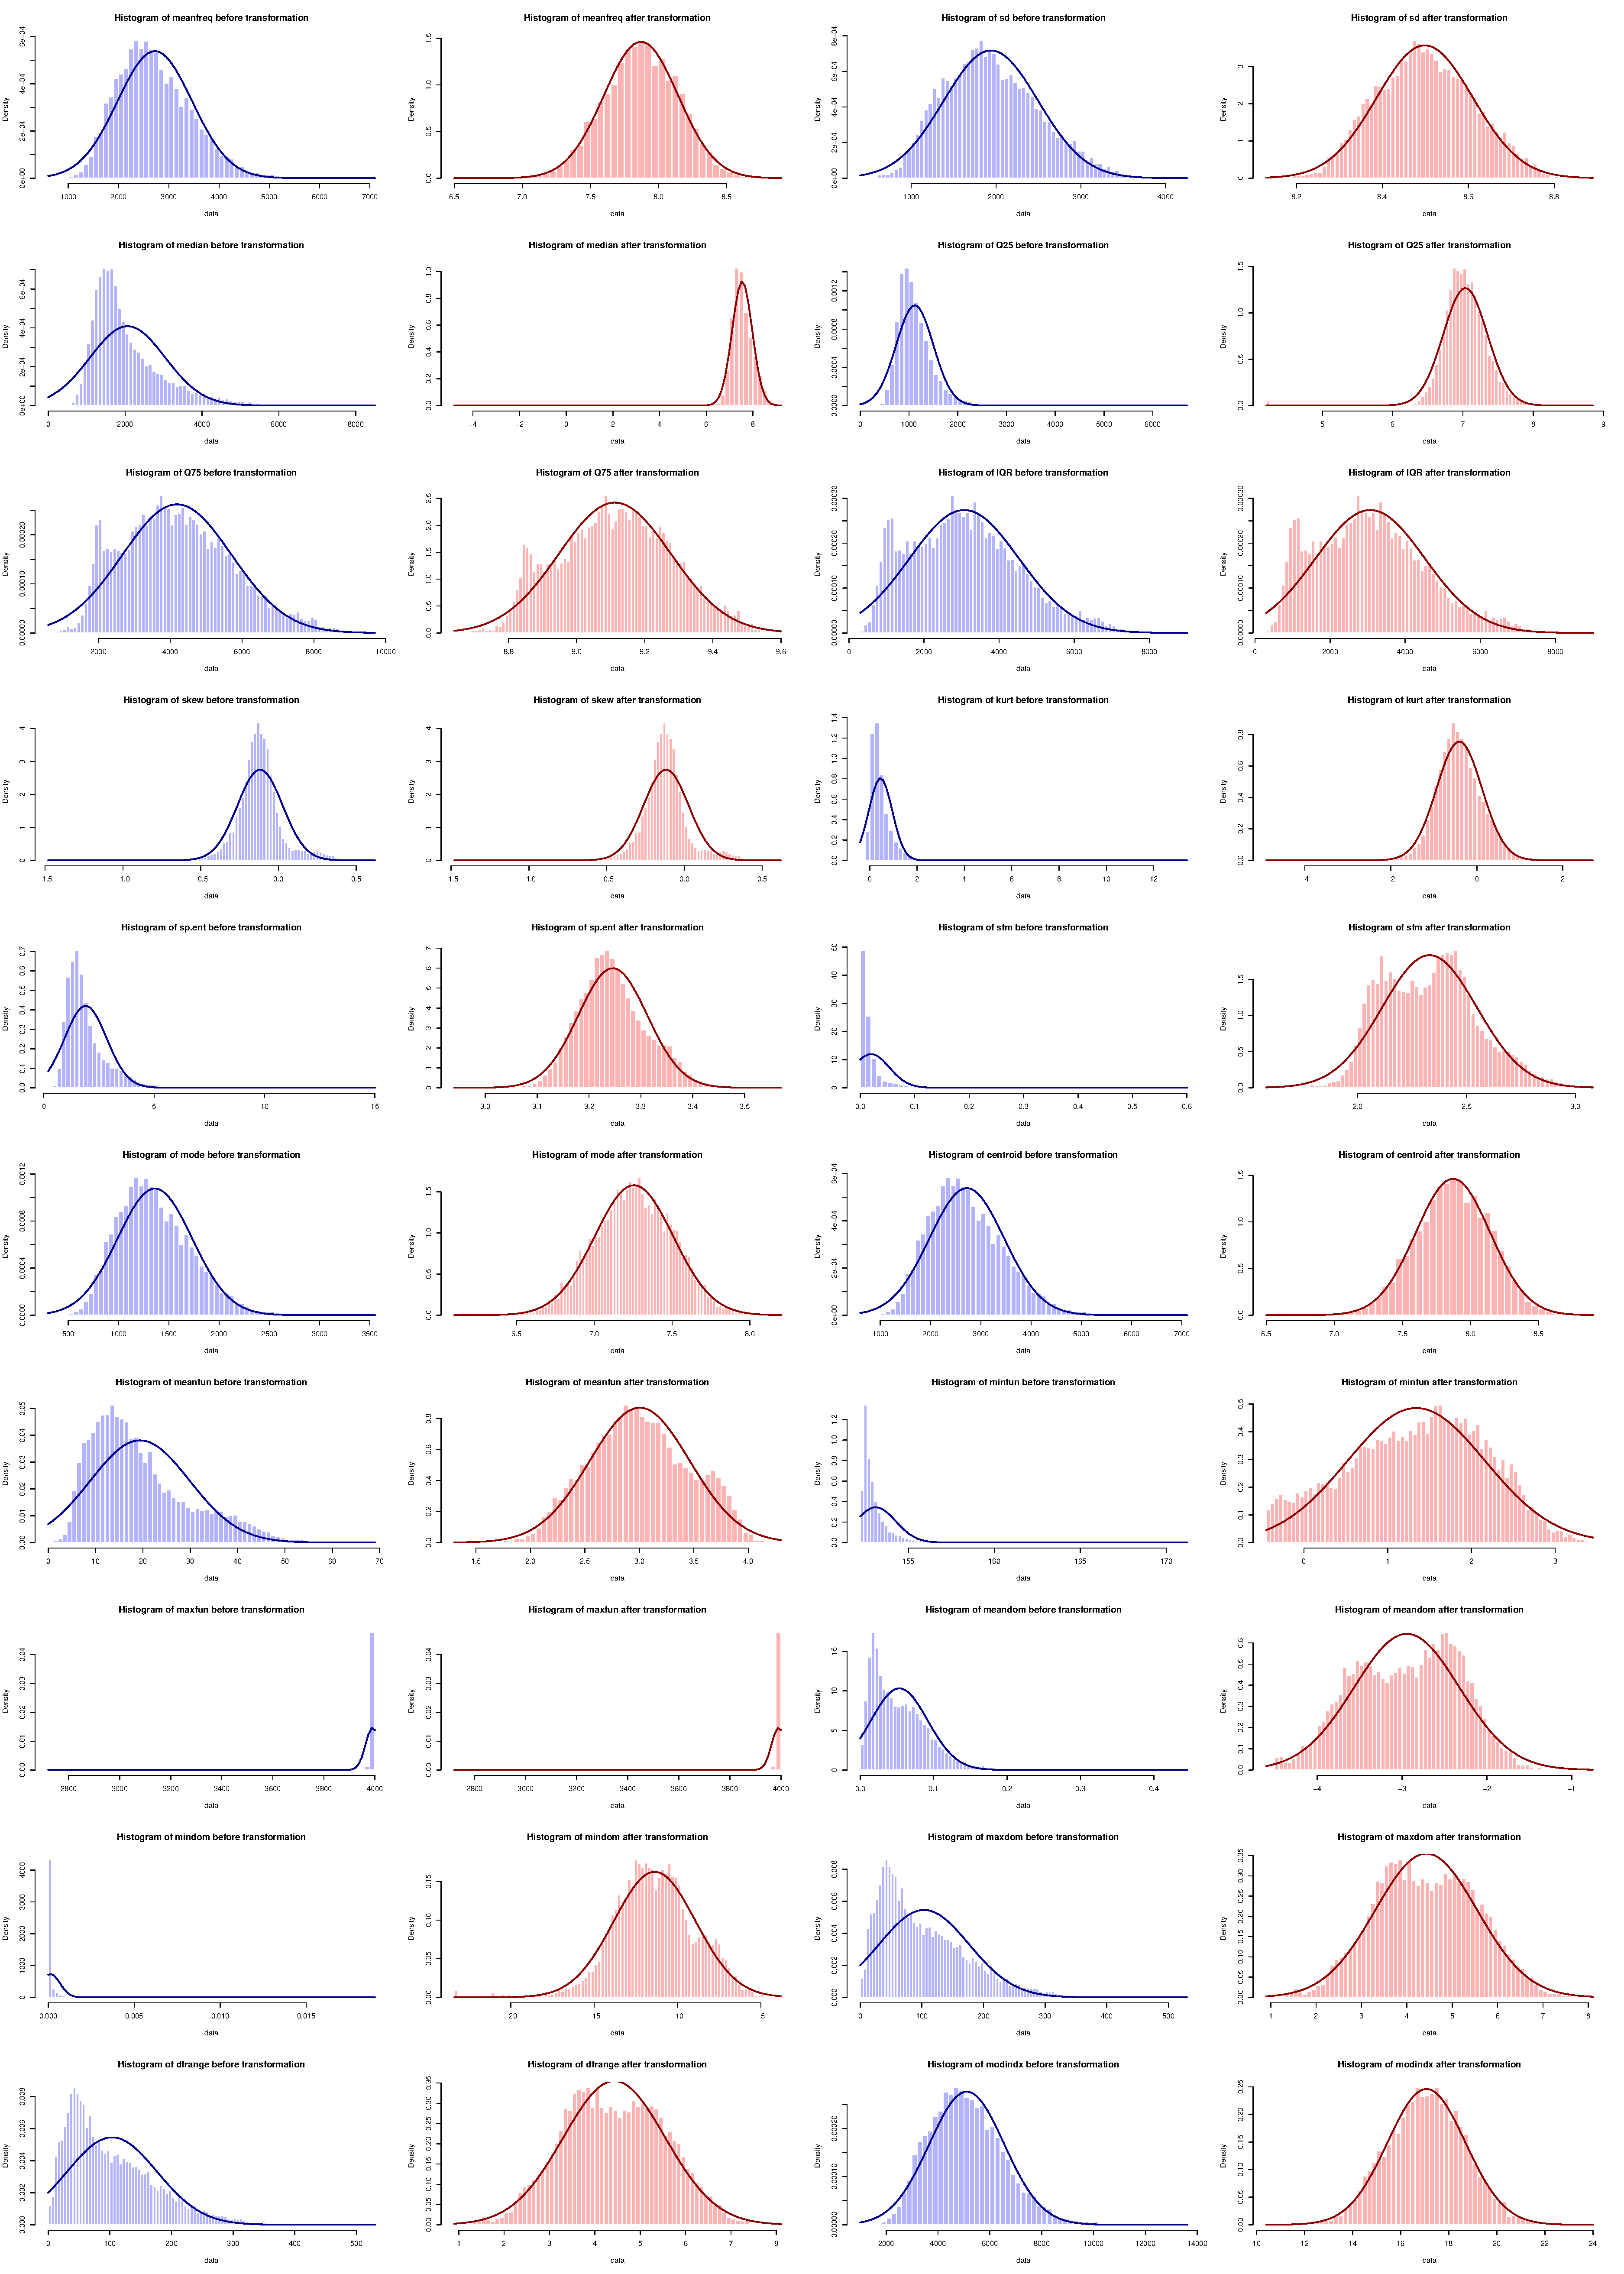
\includegraphics[width=\textwidth]{graphs/transformations_hist.pdf}
		\caption{Histogram of variables before and after transformation.}
		\label{transformation_hist}
	\end{figure}
	
	We also plot QQ-plot to visualise the normality of the variables before and after transformation in Fig. ~\ref{transformation_qq}
	\begin{figure}
		\centering
		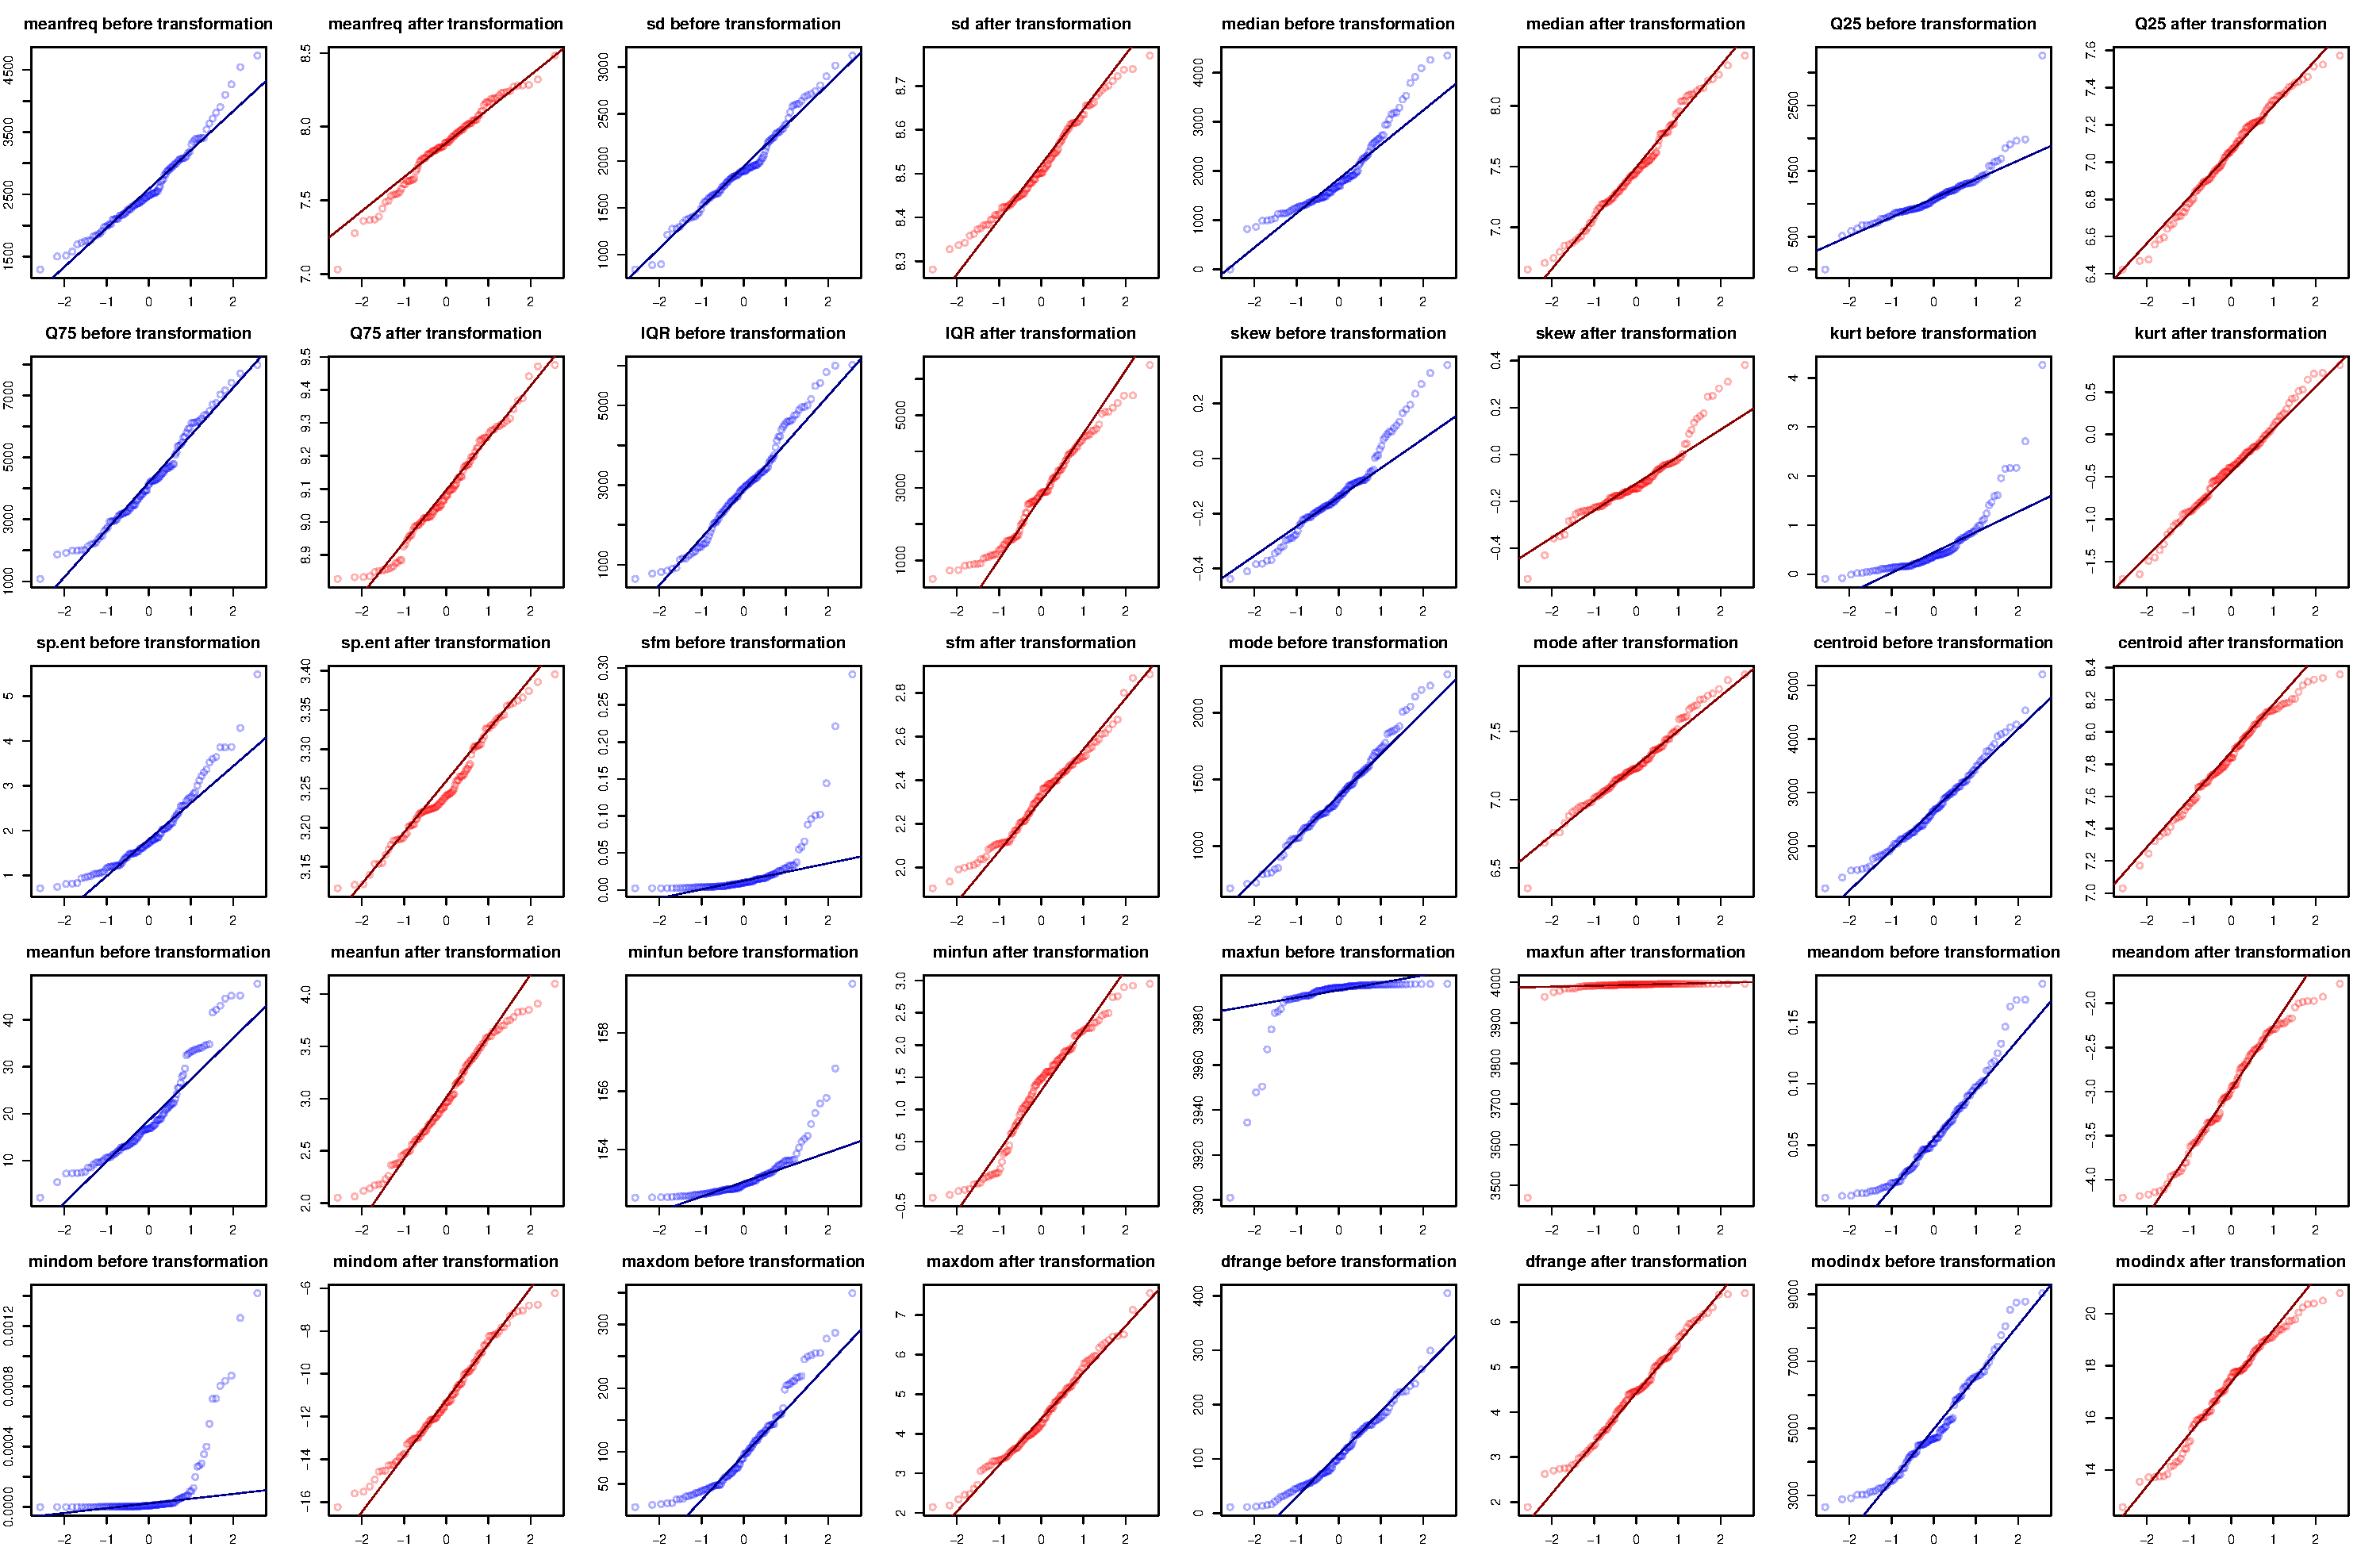
\includegraphics[width=\textwidth]{graphs/transformations_qq.pdf}
		\caption{QQ-plot of variables before and after transformation.}
		\label{transformation_qq}
	\end{figure}
	
	\subsection{Balancing Data}
	Upon initial examination, it was evident that the original data is unbalanced, as the proportion of male voice samples is significantly larger than the number of female voice samples. There were also samples categorized under unspecified gender, making it difficult to analyze. 
	
	Therefore,we balanced the gender proportions in the dataset to prevent the female data from being treated as a minority and potentially categorized as outliers. To ensure balanced representation of genders, the R script \textbf{randomly sample} data from the larger gender group to match the size of the smaller gender group. After combining the sampled rows, the dataset is examined for outliers using the Interquartile Range (IQR) method. This ensures that both genders are adequately represented in the dataset, minimizing the risk of unintentional bias during the cleaning process. 
	
	After all the preparation, there are totally 1444 observations from female and male samples. Also, 9 numerical variables and 2 categorical variables (i.e. gender and age) are retained for analysis:
	\begin{itemize}
		\item meanfreq: mean frequency (in kHz)
		\item sd: standard deviation of frequency
		\item median: median frequency (in kHz)
		\item Q25: first quantile (in kHz)
		\item Q75: third quantile (in kHz)
		\item skew: skewness
		\item sp.ent: spectral entropy
		\item sfm: spectral flatness
		\item meanfun: average of fundamental frequency measured across acoustic signal
	\end{itemize}
	
	
	\section{Data Analysis and Testing}
	
	\subsection{Data Analysis By Gender}
	
	\textbf{General steps:}
	\begin{itemize}
		\item Visualizing the data: We begin by creating a histogram to visually inspect the distribution of the data.
		\item Checking for normality: Next, we generate a QQ-plot to show whether the data follows a normal distribution.
	\end{itemize}
	If the data is normally distributed, we conduct an F-test to compare the variance of the data.
	\begin{itemize}
		\item Comparing variance using \textbf{F-test}: If the p-value from the F-test is less than 0.05, we reject the null hypothesis that the variance of the data is the same across groups. Otherwise, we do not reject the null hypothesis.
		\item Using \textbf{two sample T-test}: We proceed to perform a two-sample T-test assuming unequal variances.If the p-value from the T-test is less than 0.05, we reject the null hypothesis that the mean of the data is the same across groups. Otherwise, we do not reject the null hypothesis.
	\end{itemize}
	If the data is not normally distributed, we employ the Wilcoxon test to compare the mean of the data.
	\begin{itemize}
		\item Wilcoxon test for non-normally distributed data: If the p-value from the Wilcoxon test is less than 0.05, we reject the null hypothesis that the mean of the data is the same across groups. Additionally, by specifying "alt = less" in the Wilcoxon test, we can determine which group has a smaller mean.
	\end{itemize}
	The histogram of 9 variables of both genders are given below in Fig. ~\ref{hist_bothgender}:
	\begin{figure}
		\centering
		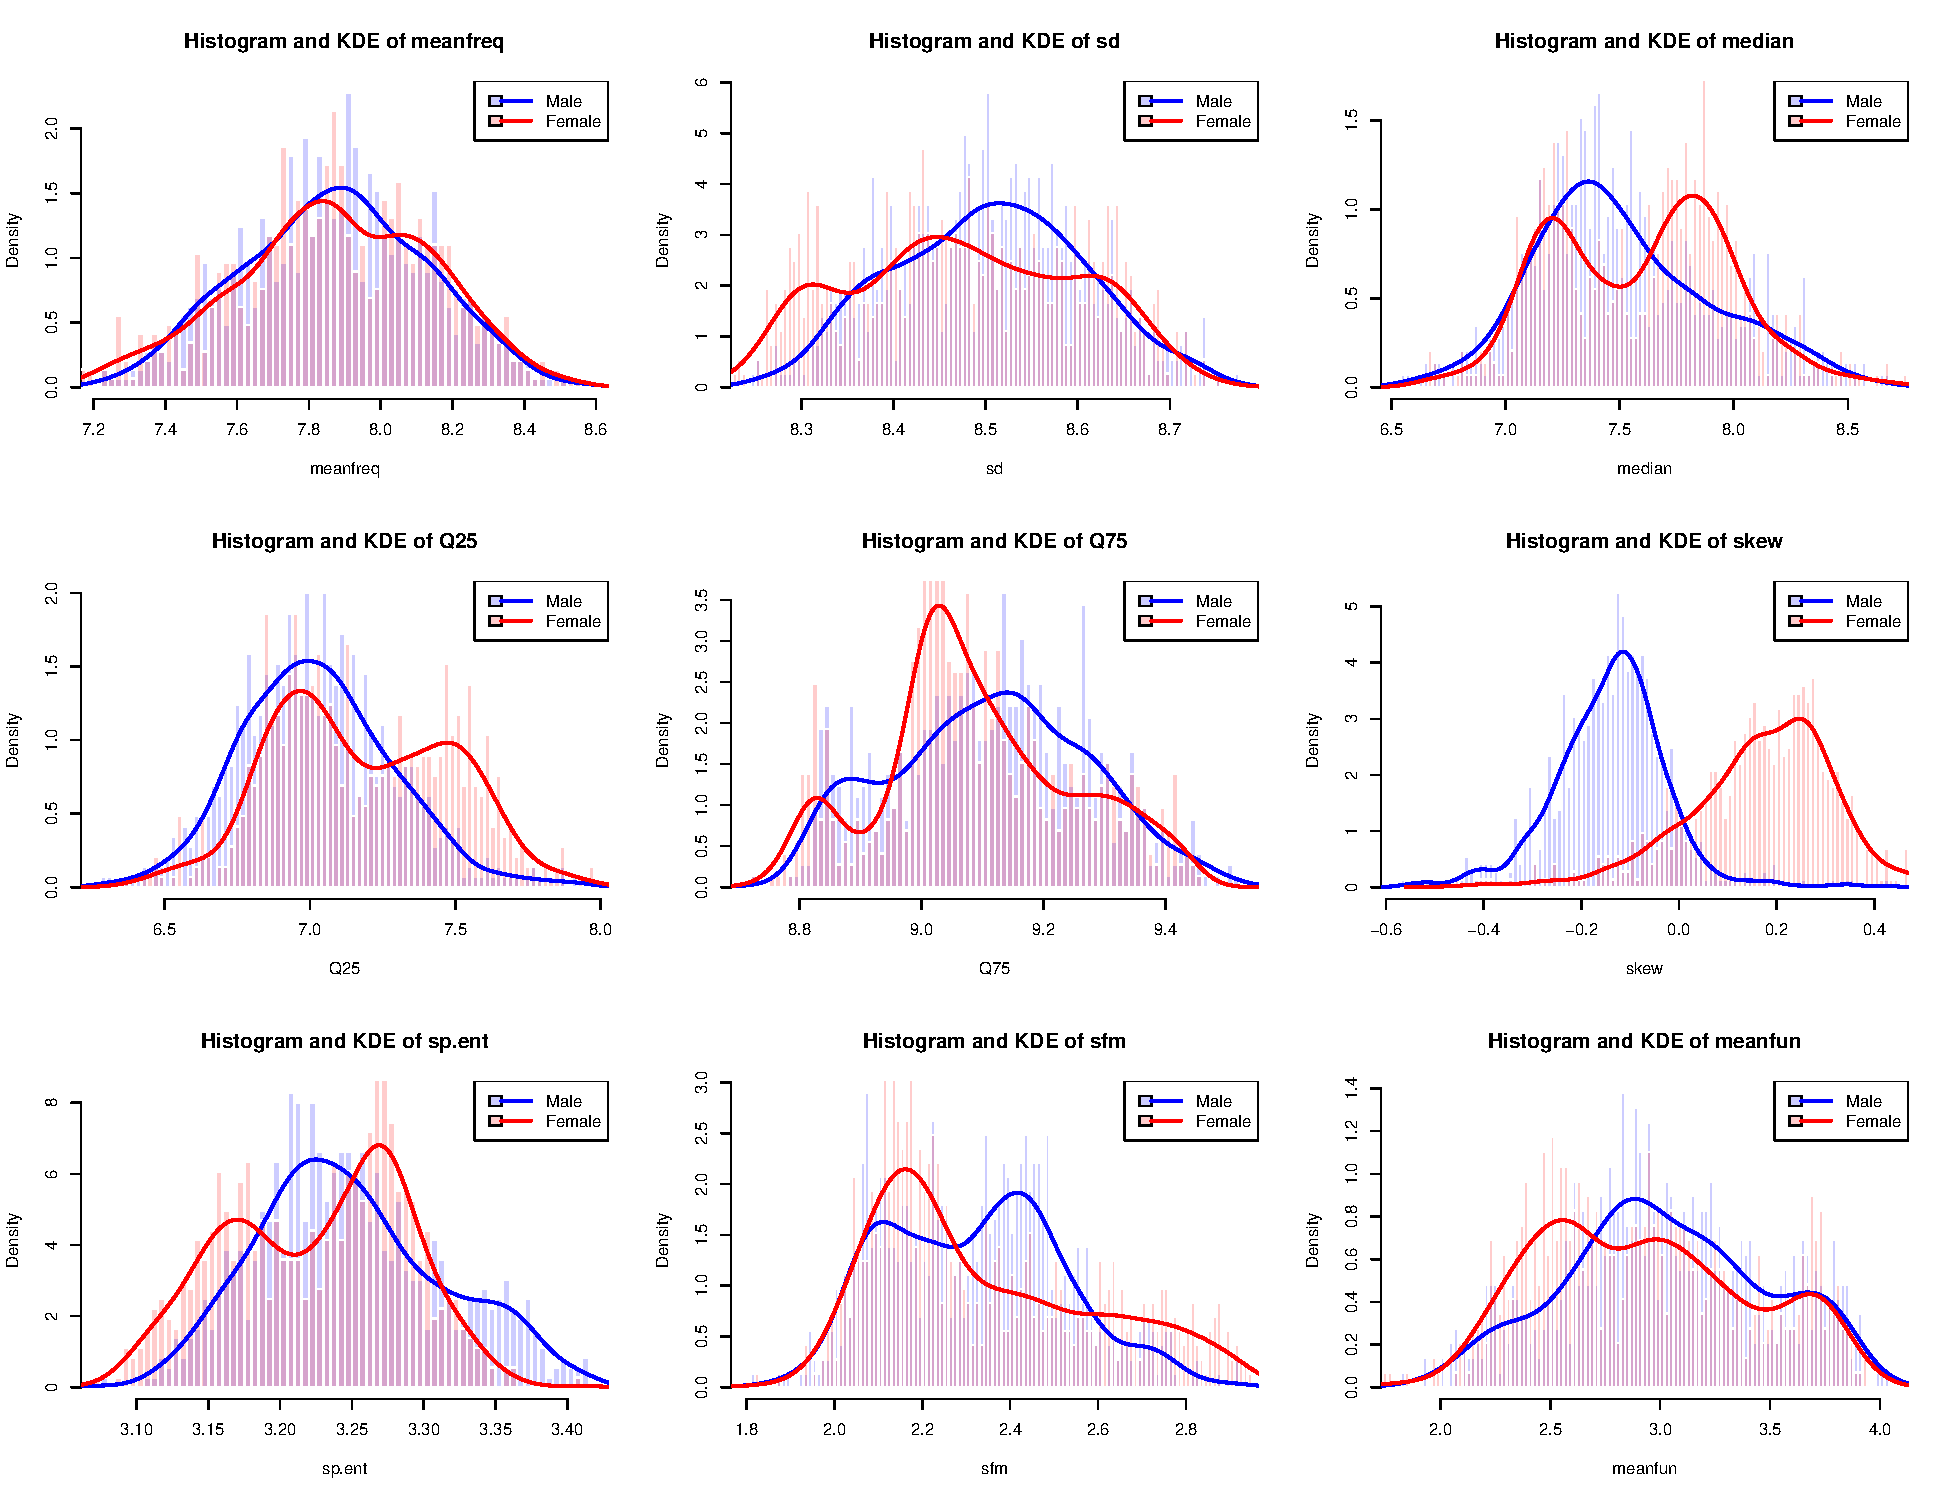
\includegraphics[width=\textwidth]{graphs/gender/visualizations.pdf}
		\caption{Histogram of variables in both genders.}
		\label{hist_bothgender}
	\end{figure}
	
	The histogram and KDEs shows noticeable differences between male and femore voices across various attributes. In general, we can observe lower frequencies (mean, median, Q25, Q75) in male voices and higher in female voices. Skewness and spectral properties like flatness and entropy also differ between those two genders. 
	
	The QQ-plot of 9 variables of male dataset are given in Fig. ~\ref{qq_male}:
	\begin{figure}
		\centering
		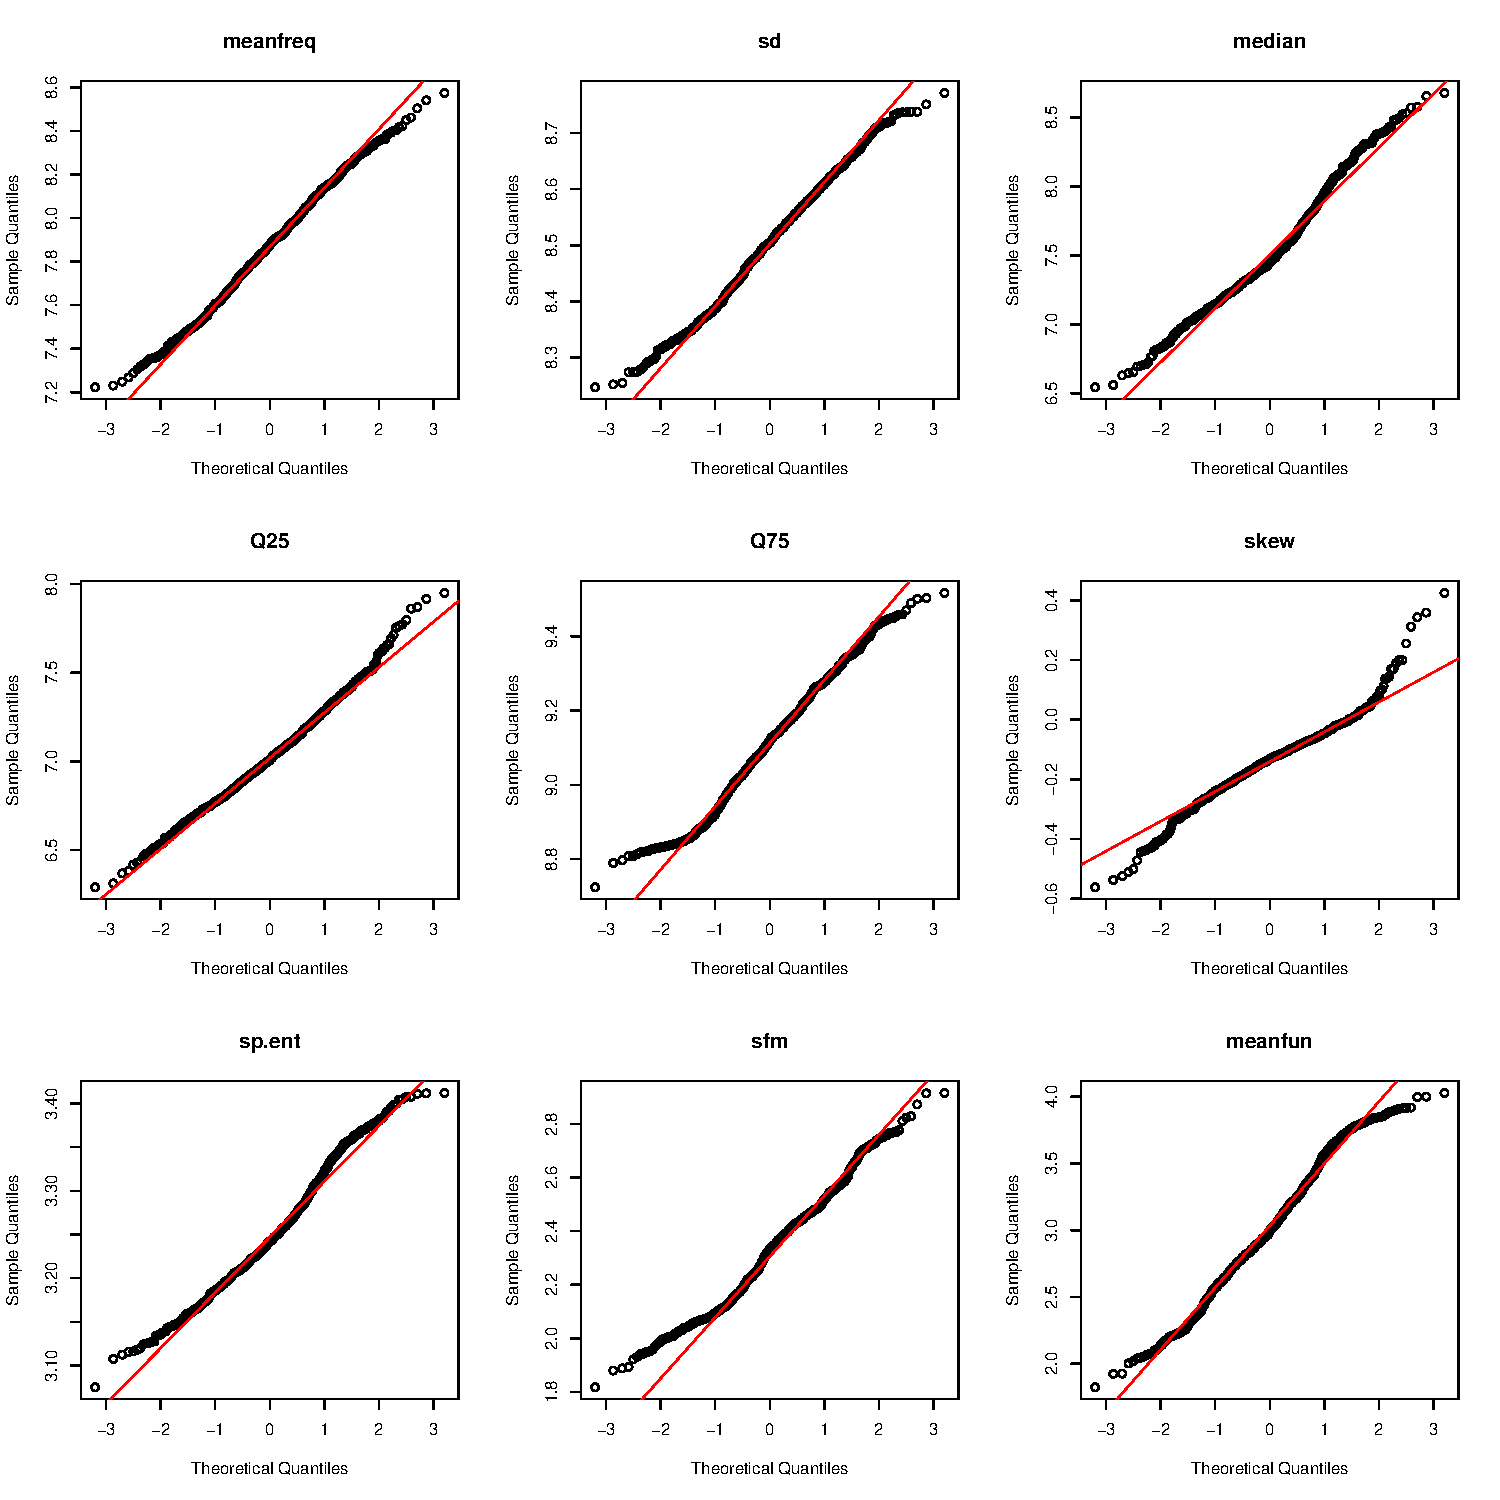
\includegraphics[width=\textwidth]{graphs/gender/qq_plot_male.pdf}
		\caption{QQ-plot of male dataset.}
		\label{qq_male}
	\end{figure}
	
	The QQ-plot of 9 variables of female dataset are given in Fig. ~\ref{qq_female}:
	\begin{figure}
		\centering
		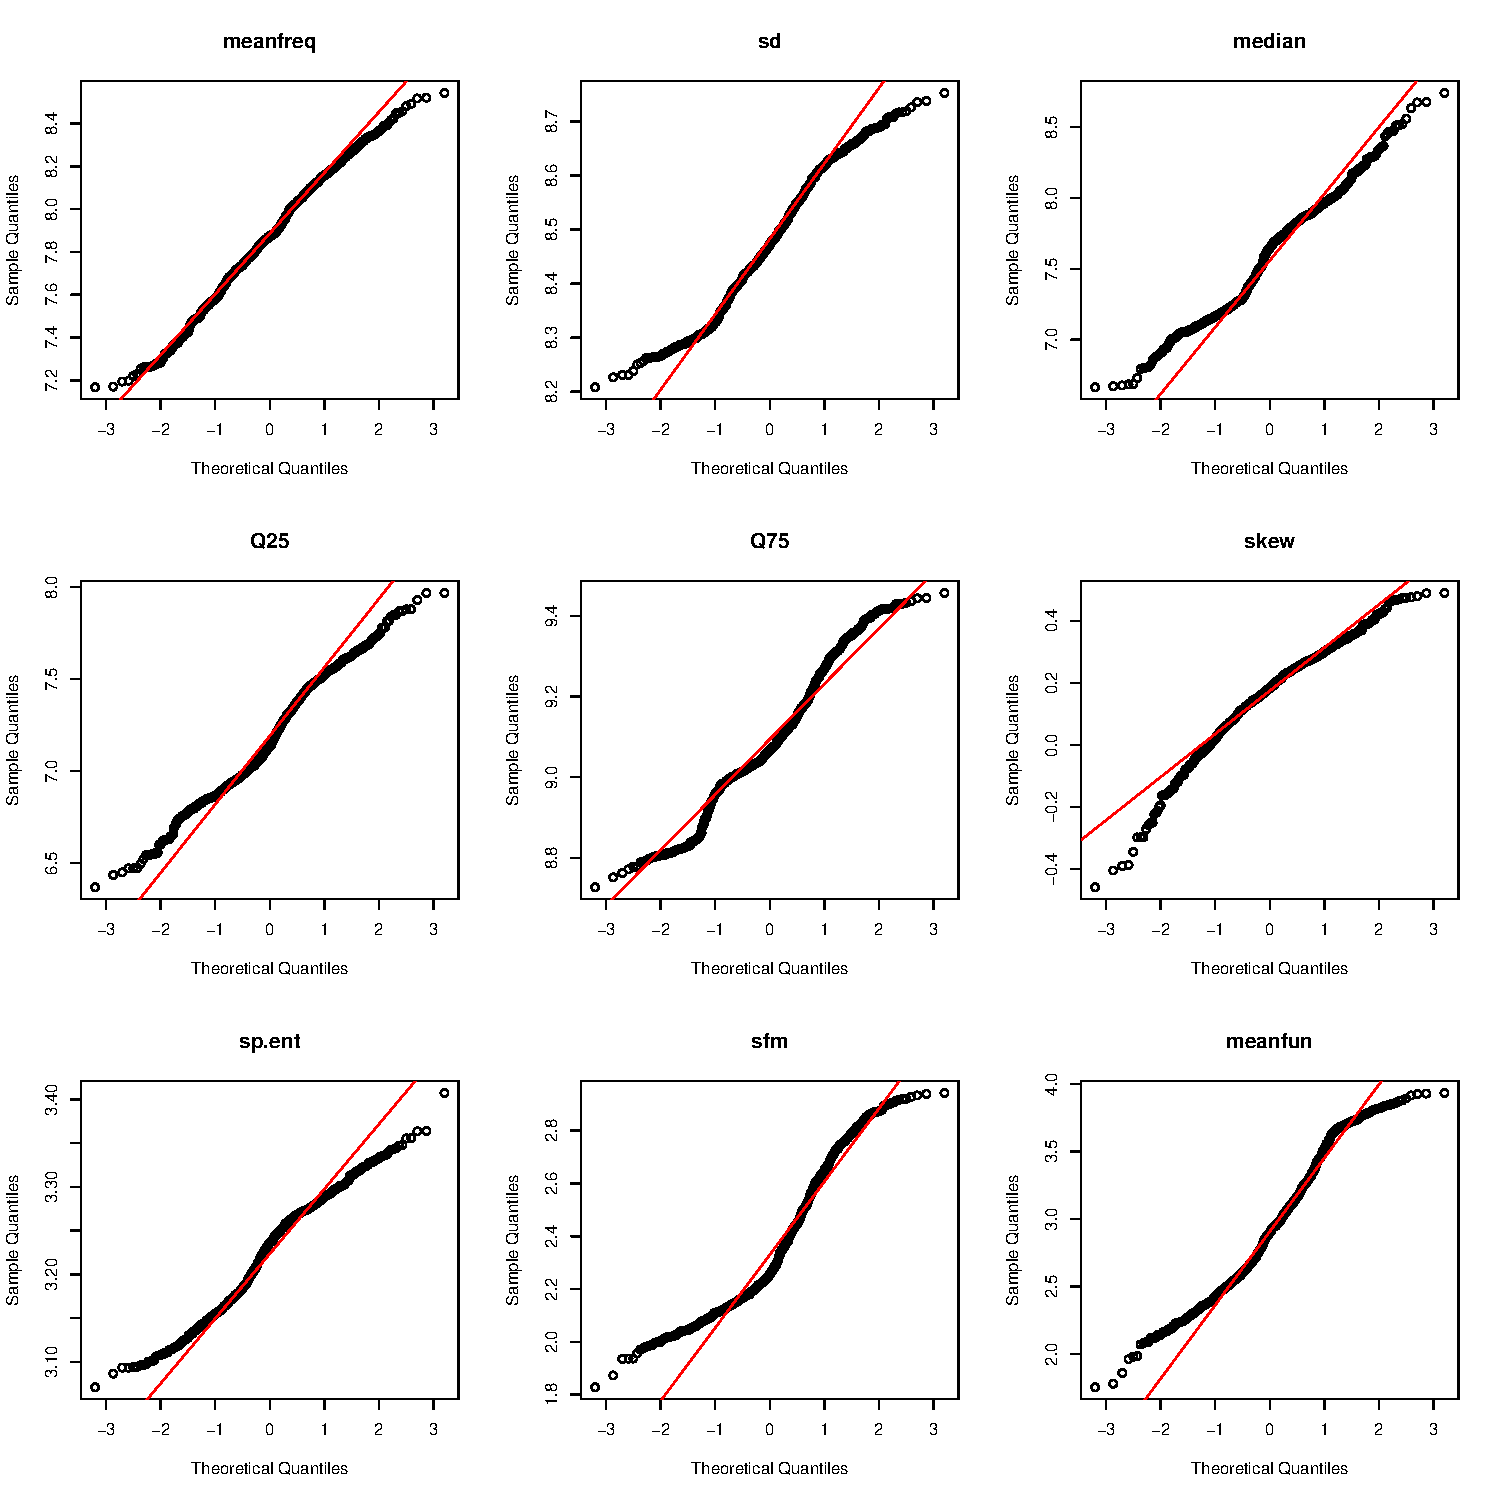
\includegraphics[width=\textwidth]{graphs/gender/qq_plot_female.pdf}
		\caption{QQ-plot of female dataset.}
		\label{qq_female}
	\end{figure}
	
	\subsection{Data Analysis By Age}
	\textbf{General steps:}
	\begin{itemize}
		\item Visualizing the data: \textbf{Boxplots} are firstly used to illustrate the distribution of mean frequency across different age groups. Each boxplot displays the median, quartiles, and outliers for each age group.
		\item Checking for normality: \textbf{Shapiro-Wilk tests} are performed on the mean frequency data within each age group to determine if the data follows a normal distribution.
		\item Comparing differences between age groups: \textbf{Kruskal-Wallis tests} are conducted to compare the mean frequency among different age groups to identify significant differences.
		\item \textbf{Pairwise Wilcoxon tests}: If significant differences are found, pairwise Wilcoxon tests are conducted to determine which age groups exhibit differences.
	\end{itemize}
	
	
	\section{Correlation}
	We visualise the correlation between variables in Fig. ~\ref{correlation_matrix}
	\begin{figure}
		\centering
		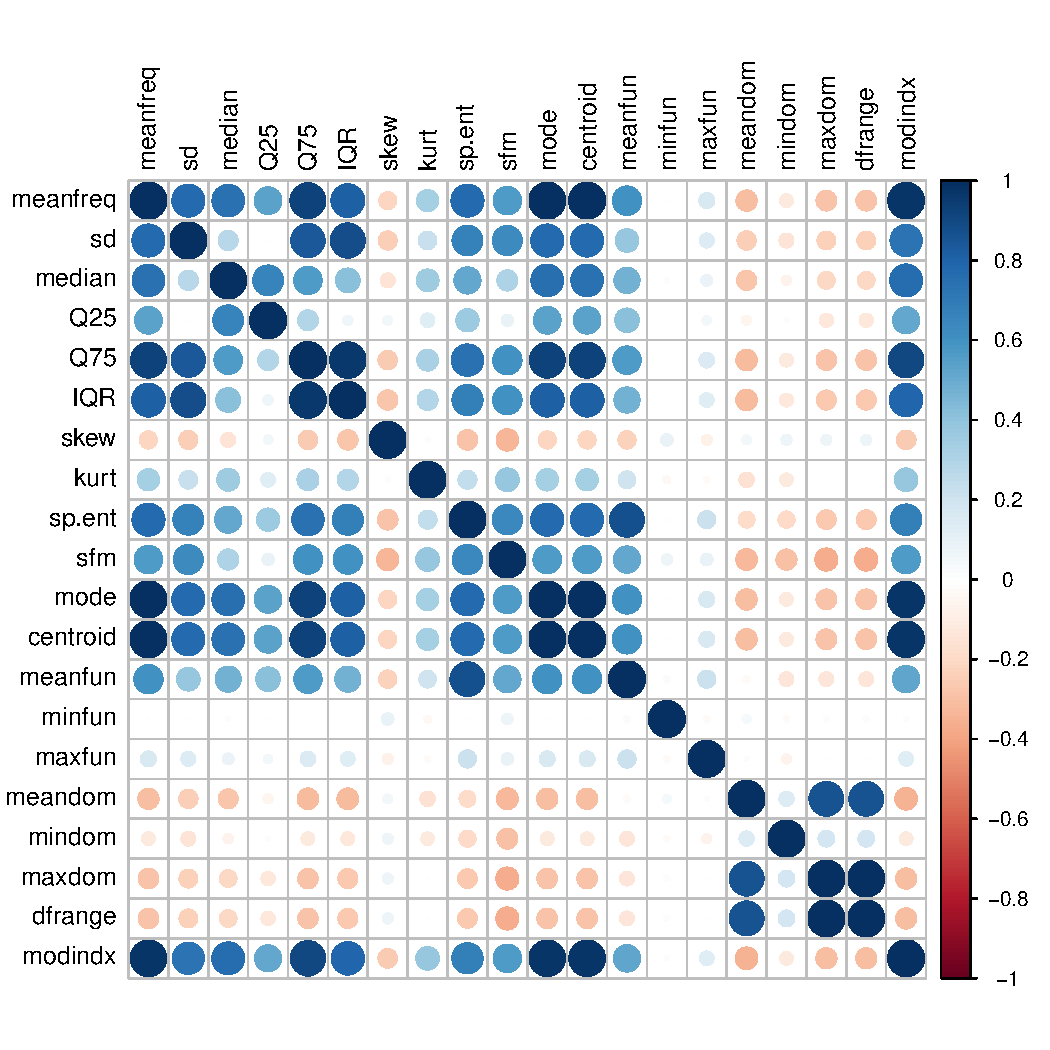
\includegraphics[width=\textwidth]{graphs/correlation_matrix.pdf}
		\caption{Correlation Matrix.}
		\label{correlation_matrix}
	\end{figure}
	
	\section{Regression Analysis}
	\subsection{Simple Linear Regression}
	\subsection{Multiple Linear Regression}
	\subsection{Logistic Regression}
	\subsection{K Nearest Neighbour}
	
	\section{Submission of papers to NeurIPS 2024}
	
	
	Please read the instructions below carefully and follow them faithfully.
	
	
	\subsection{Style}
	
	
	Papers to be submitted to NeurIPS 2024 must be prepared according to the
	instructions presented here. Papers may only be up to {\bf nine} pages long,
	including figures. Additional pages \emph{containing only acknowledgments and
		references} are allowed. Papers that exceed the page limit will not be
	reviewed, or in any other way considered for presentation at the conference.
	
	
	The margins in 2024 are the same as those in previous years.
	
	
	Authors are required to use the NeurIPS \LaTeX{} style files obtainable at the
	NeurIPS website as indicated below. Please make sure you use the current files
	and not previous versions. Tweaking the style files may be grounds for
	rejection.
	
	
	\subsection{Retrieval of style files}
	
	
	The style files for NeurIPS and other conference information are available on
	the website at
	\begin{center}
		\url{http://www.neurips.cc/}
	\end{center}
	The file \verb+neurips_2024.pdf+ contains these instructions and illustrates the
	various formatting requirements your NeurIPS paper must satisfy.
	
	
	The only supported style file for NeurIPS 2024 is \verb+neurips_2024.sty+,
	rewritten for \LaTeXe{}.  \textbf{Previous style files for \LaTeX{} 2.09,
		Microsoft Word, and RTF are no longer supported!}
	
	
	The \LaTeX{} style file contains three optional arguments: \verb+final+, which
	creates a camera-ready copy, \verb+preprint+, which creates a preprint for
	submission to, e.g., arXiv, and \verb+nonatbib+, which will not load the
	\verb+natbib+ package for you in case of package clash.
	
	
	\paragraph{Preprint option}
	If you wish to post a preprint of your work online, e.g., on arXiv, using the
	NeurIPS style, please use the \verb+preprint+ option. This will create a
	nonanonymized version of your work with the text ``Preprint. Work in progress.''
	in the footer. This version may be distributed as you see fit, as long as you do not say which conference it was submitted to. Please \textbf{do
		not} use the \verb+final+ option, which should \textbf{only} be used for
	papers accepted to NeurIPS.
	
	
	At submission time, please omit the \verb+final+ and \verb+preprint+
	options. This will anonymize your submission and add line numbers to aid
	review. Please do \emph{not} refer to these line numbers in your paper as they
	will be removed during generation of camera-ready copies.
	
	
	The file \verb+neurips_2024.tex+ may be used as a ``shell'' for writing your
	paper. All you have to do is replace the author, title, abstract, and text of
	the paper with your own.
	
	
	The formatting instructions contained in these style files are summarized in
	Sections \ref{gen_inst}, \ref{headings}, and \ref{others} below.
	
	
	\section{General formatting instructions}
	\label{gen_inst}
	
	
	
	The text must be confined within a rectangle 5.5~inches (33~picas) wide and
	9~inches (54~picas) long. The left margin is 1.5~inch (9~picas).  Use 10~point
	type with a vertical spacing (leading) of 11~points.  Times New Roman is the
	preferred typeface throughout, and will be selected for you by default.
	Paragraphs are separated by \nicefrac{1}{2}~line space (5.5 points), with no
	indentation.
	
	
	The paper title should be 17~point, initial caps/lower case, bold, centered
	between two horizontal rules. The top rule should be 4~points thick and the
	bottom rule should be 1~point thick. Allow \nicefrac{1}{4}~inch space above and
	below the title to rules. All pages should start at 1~inch (6~picas) from the
	top of the page.
	
	
	For the final version, authors' names are set in boldface, and each name is
	centered above the corresponding address. The lead author's name is to be listed
	first (left-most), and the co-authors' names (if different address) are set to
	follow. If there is only one co-author, list both author and co-author side by
	side.
	
	
	Please pay special attention to the instructions in Section \ref{others}
	regarding figures, tables, acknowledgments, and references.
	
	
	\section{Headings: first level}
	\label{headings}
	
	
	All headings should be lower case (except for first word and proper nouns),
	flush left, and bold.
	
	
	First-level headings should be in 12-point type.
	
	
	\subsection{Headings: second level}
	
	
	Second-level headings should be in 10-point type.
	
	
	\subsubsection{Headings: third level}
	
	
	Third-level headings should be in 10-point type.
	
	
	\paragraph{Paragraphs}
	
	
	There is also a \verb+\paragraph+ command available, which sets the heading in
	bold, flush left, and inline with the text, with the heading followed by 1\,em
	of space.
	
	
	\section{Citations, figures, tables, references}
	\label{others}
	
	
	These instructions apply to everyone.
	
	
	\subsection{Citations within the text}
	
	
	The \verb+natbib+ package will be loaded for you by default.  Citations may be
	author/year or numeric, as long as you maintain internal consistency.  As to the
	format of the references themselves, any style is acceptable as long as it is
	used consistently.
	
	
	The documentation for \verb+natbib+ may be found at
	\begin{center}
		\url{http://mirrors.ctan.org/macros/latex/contrib/natbib/natnotes.pdf}
	\end{center}
	Of note is the command \verb+\citet+, which produces citations appropriate for
	use in inline text.  For example,
	\begin{verbatim}
		\citet{hasselmo} investigated\dots
	\end{verbatim}
	produces
	\begin{quote}
		Hasselmo, et al.\ (1995) investigated\dots
	\end{quote}
	
	
	If you wish to load the \verb+natbib+ package with options, you may add the
	following before loading the \verb+neurips_2024+ package:
	\begin{verbatim}
		\PassOptionsToPackage{options}{natbib}
	\end{verbatim}
	
	
	If \verb+natbib+ clashes with another package you load, you can add the optional
	argument \verb+nonatbib+ when loading the style file:
	\begin{verbatim}
		\usepackage[nonatbib]{neurips_2024}
	\end{verbatim}
	
	
	As submission is double blind, refer to your own published work in the third
	person. That is, use ``In the previous work of Jones et al.\ [4],'' not ``In our
	previous work [4].'' If you cite your other papers that are not widely available
	(e.g., a journal paper under review), use anonymous author names in the
	citation, e.g., an author of the form ``A.\ Anonymous'' and include a copy of the anonymized paper in the supplementary material.
	
	
	\subsection{Footnotes}
	
	
	Footnotes should be used sparingly.  If you do require a footnote, indicate
	footnotes with a number\footnote{Sample of the first footnote.} in the
	text. Place the footnotes at the bottom of the page on which they appear.
	Precede the footnote with a horizontal rule of 2~inches (12~picas).
	
	
	Note that footnotes are properly typeset \emph{after} punctuation
	marks.\footnote{As in this example.}
	
	
	\subsection{Figures}
	
	
	\begin{figure}
		\centering
		\fbox{\rule[-.5cm]{0cm}{4cm} \rule[-.5cm]{4cm}{0cm}}
		\caption{Sample figure caption.}
	\end{figure}
	
	
	All artwork must be neat, clean, and legible. Lines should be dark enough for
	purposes of reproduction. The figure number and caption always appear after the
	figure. Place one line space before the figure caption and one line space after
	the figure. The figure caption should be lower case (except for first word and
	proper nouns); figures are numbered consecutively.
	
	
	You may use color figures.  However, it is best for the figure captions and the
	paper body to be legible if the paper is printed in either black/white or in
	color.
	
	
	\subsection{Tables}
	
	
	All tables must be centered, neat, clean and legible.  The table number and
	title always appear before the table.  See Table~\ref{sample-table}.
	
	
	Place one line space before the table title, one line space after the
	table title, and one line space after the table. The table title must
	be lower case (except for first word and proper nouns); tables are
	numbered consecutively.
	
	
	Note that publication-quality tables \emph{do not contain vertical rules.} We
	strongly suggest the use of the \verb+booktabs+ package, which allows for
	typesetting high-quality, professional tables:
	\begin{center}
		\url{https://www.ctan.org/pkg/booktabs}
	\end{center}
	This package was used to typeset Table~\ref{sample-table}.
	
	
	\begin{table}
		\caption{Sample table title}
		\label{sample-table}
		\centering
		\begin{tabular}{lll}
			\toprule
			\multicolumn{2}{c}{Part}                   \\
			\cmidrule(r){1-2}
			Name     & Description     & Size ($\mu$m) \\
			\midrule
			Dendrite & Input terminal  & $\sim$100     \\
			Axon     & Output terminal & $\sim$10      \\
			Soma     & Cell body       & up to $10^6$  \\
			\bottomrule
		\end{tabular}
	\end{table}
	
	\subsection{Math}
	Note that display math in bare TeX commands will not create correct line numbers for submission. Please use LaTeX (or AMSTeX) commands for unnumbered display math. (You really shouldn't be using \$\$ anyway; see \url{https://tex.stackexchange.com/questions/503/why-is-preferable-to} and \url{https://tex.stackexchange.com/questions/40492/what-are-the-differences-between-align-equation-and-displaymath} for more information.)
	
	\subsection{Final instructions}
	
	Do not change any aspects of the formatting parameters in the style files.  In
	particular, do not modify the width or length of the rectangle the text should
	fit into, and do not change font sizes (except perhaps in the
	\textbf{References} section; see below). Please note that pages should be
	numbered.
	
	
	\section{Preparing PDF files}
	
	
	Please prepare submission files with paper size ``US Letter,'' and not, for
	example, ``A4.''
	
	
	Fonts were the main cause of problems in the past years. Your PDF file must only
	contain Type 1 or Embedded TrueType fonts. Here are a few instructions to
	achieve this.
	
	
	\begin{itemize}
		
		
		\item You should directly generate PDF files using \verb+pdflatex+.
		
		
		\item You can check which fonts a PDF files uses.  In Acrobat Reader, select the
		menu Files$>$Document Properties$>$Fonts and select Show All Fonts. You can
		also use the program \verb+pdffonts+ which comes with \verb+xpdf+ and is
		available out-of-the-box on most Linux machines.
		
		
		\item \verb+xfig+ "patterned" shapes are implemented with bitmap fonts.  Use
		"solid" shapes instead.
		
		
		\item The \verb+\bbold+ package almost always uses bitmap fonts.  You should use
		the equivalent AMS Fonts:
		\begin{verbatim}
			\usepackage{amsfonts}
		\end{verbatim}
		followed by, e.g., \verb+\mathbb{R}+, \verb+\mathbb{N}+, or \verb+\mathbb{C}+
		for $\mathbb{R}$, $\mathbb{N}$ or $\mathbb{C}$.  You can also use the following
		workaround for reals, natural and complex:
		\begin{verbatim}
			\newcommand{\RR}{I\!\!R} %real numbers
			\newcommand{\Nat}{I\!\!N} %natural numbers
			\newcommand{\CC}{I\!\!\!\!C} %complex numbers
		\end{verbatim}
		Note that \verb+amsfonts+ is automatically loaded by the \verb+amssymb+ package.
		
		
	\end{itemize}
	
	
	If your file contains type 3 fonts or non embedded TrueType fonts, we will ask
	you to fix it.
	
	
	\subsection{Margins in \LaTeX{}}
	
	
	Most of the margin problems come from figures positioned by hand using
	\verb+\special+ or other commands. We suggest using the command
	\verb+\includegraphics+ from the \verb+graphicx+ package. Always specify the
	figure width as a multiple of the line width as in the example below:
	\begin{verbatim}
		\usepackage[pdftex]{graphicx} ...
		\includegraphics[width=0.8\linewidth]{myfile.pdf}
	\end{verbatim}
	See Section 4.4 in the graphics bundle documentation
	(\url{http://mirrors.ctan.org/macros/latex/required/graphics/grfguide.pdf})
	
	
	A number of width problems arise when \LaTeX{} cannot properly hyphenate a
	line. Please give LaTeX hyphenation hints using the \verb+\-+ command when
	necessary.
	
	\begin{ack}
		Use unnumbered first level headings for the acknowledgments. All acknowledgments
		go at the end of the paper before the list of references. Moreover, you are required to declare
		funding (financial activities supporting the submitted work) and competing interests (related financial activities outside the submitted work).
		More information about this disclosure can be found at: \url{https://neurips.cc/Conferences/2024/PaperInformation/FundingDisclosure}.
		
		
		Do {\bf not} include this section in the anonymized submission, only in the final paper. You can use the \texttt{ack} environment provided in the style file to automatically hide this section in the anonymized submission.
	\end{ack}
	
	\section*{References}
	
	
	References follow the acknowledgments in the camera-ready paper. Use unnumbered first-level heading for
	the references. Any choice of citation style is acceptable as long as you are
	consistent. It is permissible to reduce the font size to \verb+small+ (9 point)
	when listing the references.
	Note that the Reference section does not count towards the page limit.
	\medskip
	
	
	{
		\small
		
		
		[1] Alexander, J.A.\ \& Mozer, M.C.\ (1995) Template-based algorithms for
		connectionist rule extraction. In G.\ Tesauro, D.S.\ Touretzky and T.K.\ Leen
		(eds.), {\it Advances in Neural Information Processing Systems 7},
		pp.\ 609--616. Cambridge, MA: MIT Press.
		
		
		[2] Bower, J.M.\ \& Beeman, D.\ (1995) {\it The Book of GENESIS: Exploring
			Realistic Neural Models with the GEneral NEural SImulation System.}  New York:
		TELOS/Springer--Verlag.
		
		
		[3] Hasselmo, M.E., Schnell, E.\ \& Barkai, E.\ (1995) Dynamics of learning and
		recall at excitatory recurrent synapses and cholinergic modulation in rat
		hippocampal region CA3. {\it Journal of Neuroscience} {\bf 15}(7):5249-5262.
	}
	
	
	%%%%%%%%%%%%%%%%%%%%%%%%%%%%%%%%%%%%%%%%%%%%%%%%%%%%%%%%%%%%
	
	\appendix
	
	\section{Appendix / supplemental material}
	
	
	\begin{figure}
		\centering
		\fbox{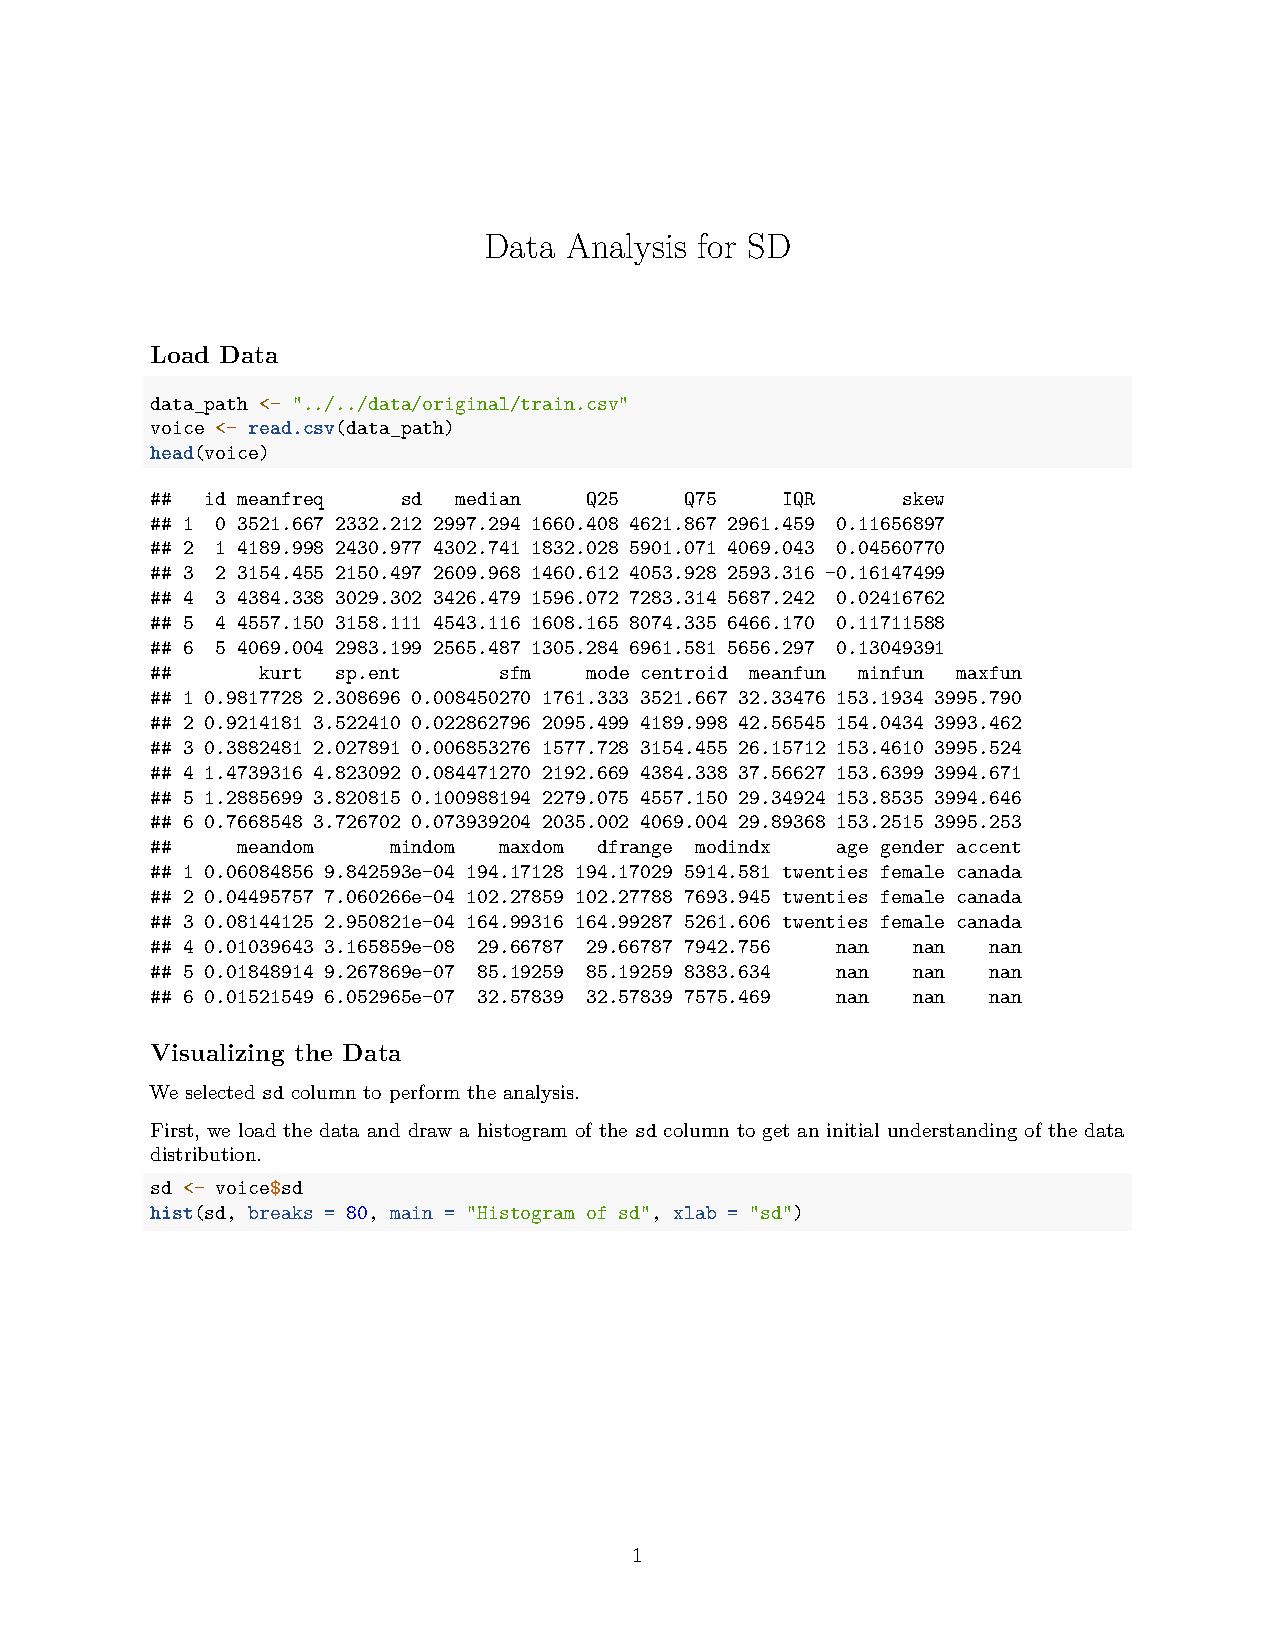
\includegraphics[page=1, width=\textwidth]{graphs/DataAnalysisSD.pdf}}
		\caption{Example Code of Data Analysis on \texttt{sd}, Page 1}
		\label{data_analysis_sd_1}
	\end{figure}
	\begin{figure}
	\centering
	\fbox{\includegraphics[page=2, width=\textwidth]{graphs/DataAnalysisSD.pdf}}
	\caption{Example Code of Data Analysis on \texttt{sd}, Page 2}
	\label{data_analysis_sd_2}
	\end{figure}
	\begin{figure}
	\centering
	\fbox{\includegraphics[page=3, width=\textwidth]{graphs/DataAnalysisSD.pdf}}
	\caption{Example Code of Data Analysis on \texttt{sd}, Page 3}
	\label{data_analysis_sd_3}
	\end{figure}
	\begin{figure}
	\centering
	\fbox{\includegraphics[page=4, width=\textwidth]{graphs/DataAnalysisSD.pdf}}
	\caption{Example Code of Data Analysis on \texttt{sd}, Page 4}
	\label{data_analysis_sd_4}
	\end{figure}
	\begin{figure}
		\centering
		\fbox{\includegraphics[page=5, width=\textwidth]{graphs/DataAnalysisSD.pdf}}
		\caption{Example Code of Data Analysis on \texttt{sd}, Page 5}
		\label{data_analysis_sd_5}
	\end{figure}


	
	
\end{document}